\documentclass[11pt,letterpaper]{article}

% ── Packages ──────────────────────────────────────────────
\usepackage[margin=1in]{geometry}
\usepackage{amsmath,amssymb,amsthm}
\usepackage{mathtools}
\usepackage{booktabs}
\usepackage{enumitem}
\usepackage{hyperref}
\usepackage[dvipsnames]{xcolor}
\usepackage{titlesec}
\usepackage{microtype}
\usepackage{parskip}
\usepackage{tikz}
\usepackage{multicol}
\usetikzlibrary{arrows.meta,positioning,calc,fit,backgrounds}

% ── Formatting ────────────────────────────────────────────
\hypersetup{colorlinks=true, linkcolor=NavyBlue, citecolor=NavyBlue, urlcolor=NavyBlue}
\titleformat{\section}{\large\bfseries}{\thesection}{1em}{}
\titleformat{\subsection}{\normalsize\bfseries}{\thesubsection}{1em}{}
\titleformat{\subsubsection}{\normalsize\itshape}{\thesubsubsection}{1em}{}

% ── Custom environments ──────────────────────────────────
\newcommand{\caveat}[1]{\par\smallskip\noindent\textcolor{gray}{\textit{Caveat:} #1}\smallskip}
\newcommand{\pp}{\,\text{pp}}

% ── Math shortcuts ────────────────────────────────────────
\newcommand{\bfp}{\mathbf{p}}
\newcommand{\bfz}{\mathbf{z}}
\newcommand{\bfy}{\mathbf{y}}
\newcommand{\bfd}{\mathbf{d}}
\newcommand{\bfb}{\mathbf{b}}
\newcommand{\cS}{\mathcal{S}}
\newcommand{\cM}{\mathcal{M}}
\newcommand{\R}{\mathbb{R}}

\begin{document}

% ── Title ─────────────────────────────────────────────────
\begin{center}
{\LARGE\bfseries Neural Field Perceiver}\\[6pt]
{\large Cross-Patient Speech Decoding from Intra-Operative $\mu$ECoG\\via Reprojection-Supervised Spatial Alignment}\\[12pt]
{\normalsize Ben Tang \quad\textbar\quad Greg Cogan Lab, Duke University}\\[4pt]
{\normalsize April 2026 \quad\textbar\quad Version 2 (Comprehensive)}
\end{center}

\medskip\noindent\rule{\textwidth}{0.4pt}\medskip

\noindent This document is the complete technical reference for the Neural Field Perceiver project. It unifies the theoretical problem framing, cross-disciplinary foundations from 3D computer vision, the full architecture specification, uncertainty estimation, and the experimental plan. Claims throughout are categorized as \textbf{externally established} (published literature), \textbf{internally observed} (our experiments), or \textbf{working hypotheses} (plausible but unverified).

\tableofcontents
\newpage


%% ====================================================================
%%  PART I: PROBLEM FRAMING
%% ====================================================================

\part{Problem Framing}

\section{The Physical Problem}

Each patient's micro-electrocorticography ($\mu$ECoG) array is a \textbf{sparse spatial sample} of neural activity over the cortical surface during speech production. The array is placed subdurally over left ventral sensorimotor cortex (vSMC) during surgery, and its position in standardized brain space (MNI-152) is determined post-hoc via electrode reconstruction (BioImage Suite for DBS patients, Brainlab for tumor patients).

\subsection{The cortical surface, not free 3D space}

The cortex is a folded two-dimensional sheet, not a volume. Let $\cS$ denote the cortical surface embedded in $\R^3$. The high-gamma analytic amplitude (HGA, 70--150\,Hz envelope) is a function on this surface:
\begin{equation}
a: \cS \times \R \to \R
\end{equation}

For patient $i$ with $N_i$ electrodes at cortical surface positions $\{\bfp_j^{(i)}\}_{j=1}^{N_i} \subset \cS$, we observe:
\begin{equation}\label{eq:observation}
\boxed{d_j^{(i)}(t) = a\bigl(\bfp_j^{(i)},\; t\bigr) + \epsilon_j^{(i)}(t)}
\end{equation}
where $\epsilon$ captures measurement noise, electrode impedance variation, and sub-electrode-scale neural activity not resolved by the ${\sim}2$\,mm contact spacing.

In practice, we approximate cortical surface positions with 3D MNI coordinates: $\bfp_j^{(i)} \approx (x_j^{(i)}, y_j^{(i)}, z_j^{(i)})_{\text{MNI}}$. This approximation has two consequences:

\begin{enumerate}[leftmargin=2em]
\item \textbf{Euclidean distance in MNI space does not equal geodesic distance on the cortical surface.} Two electrodes 3\,mm apart in MNI may sit on opposite banks of a sulcus, making them functionally distant. For $\mu$ECoG arrays on exposed cortex, the local patch under the array is approximately planar, so within-array Euclidean distances are reasonable. Cross-patient comparisons at larger scales are more affected by folding geometry.

\item \textbf{Surface-based coordinates} (e.g., projection to \texttt{fsaverage}) would better respect cortical geometry than volumetric MNI coordinates. Whether surface reconstructions exist for our patients depends on the BioImage Suite\,/\,Brainlab outputs available.
\end{enumerate}

\textbf{The decoding problem.} Given observations $\{d_j^{(i)}(t)\}$ at approximately known surface positions, infer the phoneme sequence $\bfy = (y_1, y_2, y_3)$ that produced the spatiotemporal pattern.

\textbf{The cross-patient problem.} Train on patients $\{1, \ldots, K\}$ and decode for a held-out patient $K{+}1$ whose electrodes sample the cortical surface at \emph{different positions}. The observations are not aligned: electrode $j$ on patient $i$ and electrode $j$ on patient $i'$ correspond to different cortical locations.

\subsection{What makes this hard}

\begin{table}[h]
\centering\small
\begin{tabular}{@{}lll@{}}
\toprule
\textbf{Factor} & \textbf{Quantity} & \textbf{Implication} \\
\midrule
Electrodes per patient & 63--201 & Sparse sampling of the cortical field \\
Electrode spacing & ${\sim}2$\,mm & Resolves individual gyral columns \\
Array offset across patients & 15--25\,mm in MNI & Different cortical regions sampled \\
Array rotation & Variable & Channel indices meaningless across patients \\
Correspondence uncertainty & Several mm & Coordinate-based alignment is approximate \\
Cortical folding variability & Patient-specific & Sulcal geometry differs across individuals \\
Tumor mass effect (subset) & Variable & Macroscopic warping in 6 of 12 patients \\
Trials per patient & 46--178 & Small-data regime for supervised learning \\
Total utterance per patient & ${\sim}1$\,min & Insufficient for single-patient SSL \\
Phoneme vocabulary & 9 classes $\times$ 3 positions & 27-way classification at each trial \\
\bottomrule
\end{tabular}
\end{table}


\section{The Shared Dynamics Hypothesis}

Cross-patient decoding is only possible if the cortical field $a(\bfp, t)$ shares structure across patients. We decompose:
\begin{equation}\label{eq:decomposition}
\boxed{a^{(i)}(\bfp, t) = f\bigl(T_i(\bfp),\; t;\; \bfy\bigr) + r^{(i)}(\bfp, t)}
\end{equation}
where:
\begin{itemize}[leftmargin=2em]
\item $f(\cdot, t; \bfy)$ is the \textbf{shared neural field}---the spatiotemporal pattern that phoneme sequence $\bfy$ produces in canonical cortical space.
\item $T_i: \cS_i \to \cS_{\text{canonical}}$ is a \textbf{patient-specific spatial transform} mapping each patient's cortical surface to a canonical reference. MNI normalization is our estimate of $T_i$, but it is imperfect.
\item $r^{(i)}(\bfp, t)$ is a \textbf{patient-specific residual} capturing individual neural organization, signal characteristics, and functional plasticity.
\end{itemize}
The viability of cross-patient decoding depends on the ratio $\|f\| / \|r^{(i)}\|$ at the spatial resolution accessible to our measurements and alignment procedure.

\subsection{Evidence for shared dynamics}

\subsubsection{Externally established (published literature)}

\textbf{Per-patient input layers + shared temporal backbone is the optimal transfer architecture.} Singh et al.\ (2025) demonstrate group training with $N{=}25$ sEEG patients: per-patient Conv1D + shared BiLSTM ($2{\times}64$), frozen shared backbone + fine-tuned per-patient layers yields PER 0.49 vs.\ 0.57 single-subject ($p{<}0.001$). Willett et al.\ (2023) use per-day affine input layer ($256{\to}256$) + shared 5-layer GRU (512 hidden) for day-to-day BCI transfer.

\caveat{Singh's data regime is ${\sim}60$\,min/patient (vs.\ our ${\sim}1$\,min); Conv1D hyperparameters are unreported. Willett is $N{=}1$ with ${\sim}40$\,min/day. The architectural pattern transfers; the hyperparameters do not.}

\textbf{Articulatory somatotopy in vSMC is reproducible within individuals.} Metzger et al.\ (2023) show somatotopic organization of speech articulators in one patient with chronic ECoG (253 channels): labial, front tongue, back tongue, and vocalic representations are spatially organized ($p{<}0.0001$), preserved even after 18 years of anarthria, suggesting the organization is intrinsic to motor cortex circuitry.

\caveat{$N{=}1$ chronic implant. Cross-patient spatial consistency is inferred from anatomical uniformity but not directly measured in any paper in our corpus.}

\textbf{Articulatory features are a robust encoding basis in vSMC.} Wu et al.\ (2025) reconstruct speaker-invariant articulatory features from HD-ECoG over vSMC (PCC 0.75--0.80, $N{=}3$), including one intra-operative patient (PCC\,=\,0.76). The claim that articulatory features are ``more robustly encoded than acoustic features'' is attributed by Wu to Chartier (2018), Conant (2018), and Anumanchipalli (2019).

\textbf{MNI coordinates enable cross-patient ECoG transfer.} Chen et al.\ (2025, SwinTW) use MNI coordinates and ROI embeddings as positional information across 43 ECoG + 9 sEEG subjects, reporting mean PCC\,=\,0.765 on unseen participants in cross-validation.

\caveat{Standard ECoG has ${\sim}10$\,mm spacing, comparable to inter-subject correspondence uncertainty. Our $\mu$ECoG spacing (${\sim}2$\,mm) is finer, meaning coordinates may encode global array position but not resolve within-array relationships.}

\textbf{Motor cortex neural manifold structure is preserved across individuals.} Safaie et al.\ (2023, \textit{Nature Neuroscience}) show that motor cortex population dynamics during reaching are geometrically similar across different monkeys. Separately, Gallego et al.\ (2020, \textit{Nature Neuroscience}) establish that low-dimensional manifold dynamics are preserved within individuals across long time periods, even as recorded neurons change---evidence for temporal stability of latent dynamics.

\caveat{Safaie concerns limb motor cortex in non-human primates. Gallego is within-individual. The extension to cross-individual speech motor cortex is plausible but untested.}

\textbf{Consistent articulatory somatotopy across participants.} Bouchard et al.\ (2013, \textit{Nature}) used high-density ECoG to demonstrate reproducible articulatory maps in vSMC across 3 participants. Anumanchipalli et al.\ (2019, \textit{Nature}) reconstructed continuous articulatory trajectories from motor cortex.

\subsubsection{Internally observed (our experiments)}

\textbf{Cross-patient supervised transfer works at this data scale.} Our LOPO pipeline (per-patient SpatialConv + shared BiGRU backbone, 9 source patients) achieves PER\,=\,0.762 on held-out S14, compared to per-patient PER\,=\,0.737 (grouped-by-token CV). This is direct evidence that decodable shared structure exists in~$f$.

\textbf{Articulatory bottleneck head improves LOPO decoding.} Projecting to a 15-dimensional phonological feature space via a fixed linguistic matrix outperforms a flat CE head for cross-patient decoding, consistent with $f$ being organized along articulatory feature dimensions.

\textbf{55 experiments on S14 converge to PER 0.750--0.780.} Across supervised, SSL, domain adaptation (DANN, CORAL, CCA), self-training, and knowledge distillation paradigms. See Section~\ref{sec:wall} for interpretation.

\textbf{SSL features carry partial structure.} JEPA features + LP-FT achieve PER\,=\,0.797 (vs.\ 0.854 with basic evaluation). Supervised features with the same recipe achieve 0.737. All SSL methods fail at current data scale but feature geometry is non-trivial.

\subsubsection{Working hypotheses (plausible but unverified)}

The ${\sim}0.76$ PER convergence on S14 reflects (in part) a spatial alignment bottleneck. This has not been isolated from target-data scarcity, measurement noise, or S14-specific effects.

MNI coordinate-based spatial alignment will improve decoding. The practical gain depends on registration accuracy, model architecture, and whether spatial alignment is binding.

Cross-task data pooling (Duraivel 2025 pseudoword repetition, same 9 phonemes, 3 overlapping patients) is a high-value, low-risk path to more data.


\section{The Neural Manifold Connection}\label{sec:manifold}

\subsection{Two views of the same phenomenon}

The cortical field model (Section~2) and the neural manifold hypothesis describe the same system at different levels:
\begin{itemize}[leftmargin=2em]
\item \textbf{The field view} (spatial): Activity $a(\bfp, t)$ is a function on the cortical surface. Each electrode samples this field at a known position.
\item \textbf{The manifold view} (population): The vector of all electrode activities $\bfd(t) = [d_1(t), \ldots, d_N(t)]$ lies on a low-dimensional manifold $\cM \subset \R^N$. Motor behavior corresponds to trajectories on $\cM$.
\end{itemize}

The bridge is a \textbf{latent state variable}. Let $\bfz(t) \in \R^k$ be the low-dimensional articulatory state---the configuration of the vocal tract at time $t$. Each electrode's activity is determined by \emph{where it sits} on the cortical surface and \emph{what the articulatory state is}:
\begin{equation}\label{eq:obs-function}
\boxed{d_j^{(i)}(t) = g\bigl(\bfp_j^{(i)},\; \bfz(t)\bigr) + \epsilon_j^{(i)}(t)}
\end{equation}
where $g: \cS \times \R^k \to \R$ is a \textbf{shared observation function} mapping (cortical position, articulatory state) to neural activity. This is the somatotopic map made explicit: electrodes over lip motor cortex respond to lip-state variables; electrodes over tongue motor cortex respond to tongue-state variables.

The dynamics on the manifold are determined by the phoneme sequence:
\begin{equation}\label{eq:dynamics}
\dot{\bfz}(t) = h\bigl(\bfz(t);\; \bfy\bigr)
\end{equation}

\subsection{The factorization is the key insight}

Combining the shared dynamics hypothesis with the manifold hypothesis: the shared field $f(\bfp, t; \bfy)$ factorizes as $g(\bfp, \bfz(t))$, separating space from time through a low-dimensional bottleneck. Instead of learning an arbitrary spatiotemporal function, the model learns:
\begin{enumerate}[leftmargin=2em]
\item A spatial function $g$: how each brain position encodes articulatory features (the somatotopic map).
\item A dynamical system $h$: how the articulatory state evolves during speech.
\end{enumerate}

\subsection{Articulatory manifold dimensionality}

The manifold has physical meaning corresponding to vocal tract configuration. For our 9 phonemes, the contrasts that distinguish the inventory:

\begin{table}[h]
\centering\small
\begin{tabular}{@{}llc@{}}
\toprule
\textbf{Contrast} & \textbf{Phonemes distinguished} & \textbf{Dim.} \\
\midrule
Place of articulation & labial (b,p,v) vs.\ velar (g,k) & ${\sim}2$ \\
Manner & stop vs.\ fricative vs.\ vowel & ${\sim}2$ \\
Voicing & voiced (b,g,v) vs.\ voiceless (k,p) & ${\sim}1$ \\
Vowel height & low (a,\ae) vs.\ high (i,u) & ${\sim}1$ \\
Vowel backness & front (\ae,i) vs.\ back (a,u) & ${\sim}1$ \\
\midrule
\textbf{Effective manifold dimension} & & $\mathbf{{\sim}5\text{--}8}$ \\
\bottomrule
\end{tabular}
\end{table}

\noindent This is far below the electrode count (63--201), consistent with massive oversampling of a low-dimensional manifold. The decoding problem reduces to: given sparse samples of $g(\bfp, \bfz)$ at known positions~$\bfp$, infer the latent trajectory $\bfz(t)$ and classify the phoneme sequence.

\subsection{Cross-patient transfer as manifold alignment}

Each patient's electrode array gives a different \textbf{projection} of the shared manifold:
\begin{equation}\label{eq:projection}
\bfd^{(i)}(t) \approx W^{(i)} \bfz(t) + \boldsymbol{\epsilon}^{(i)}
\end{equation}
where $W^{(i)} \in \R^{N_i \times k}$ is determined by which cortical positions the electrodes sample. Different patients have different $W^{(i)}$ because they have different electrode positions---different projections of the same underlying manifold.

Existing alignment methods (CCA, Procrustes, CORAL) attempt to align these projections post-hoc. All failed in our experiments. MNI coordinates offer an alternative: \textbf{aligning the projections a priori} by providing the geometric relationship between electrode positions.

The key question is whether inter-subject correspondence uncertainty (several mm) is small enough relative to the somatotopic map scale (${\sim}15$--$20$\,mm) that MNI coordinates provide useful alignment.


\section{Decomposing Cross-Patient Variation}

\subsection{The spatial transform $T_i$}

The primary source of cross-patient variation is \textbf{geometric}: different electrode positions sample different regions of the shared field. The transform $T_i$ decomposes:
\begin{equation}\label{eq:transform}
T_i(\bfp) = A_i \cdot \bfp + \bfb_i + \delta_i(\bfp)
\end{equation}
\begin{itemize}[leftmargin=2em]
\item $A_i \in \R^{3 \times 3}$: rigid or affine transform (rotation, scaling). MNI normalization estimates this.
\item $\bfb_i \in \R^3$: translation (15--25\,mm array placement offset).
\item $\delta_i(\bfp)$: nonlinear residual---sulcal geometry, local folding, and for tumor patients, \textbf{macroscopic warping from mass effect}. Tumor displacement is a geometric mapping error, not signal noise: it physically displaces the somatotopic map relative to skull-based coordinates.
\end{itemize}

\subsection{Inter-subject correspondence uncertainty}

The commonly cited ``${\sim}5$\,mm'' is not a stable physical constant. The actual uncertainty has multiple sources:

\begin{enumerate}[leftmargin=2em]
\item \textbf{Native-space electrode localization}: Sub-millimeter accuracy---relatively precise.
\item \textbf{Brain shift correction}: Intra-operative brain shift (craniotomy, CSF drainage, gravity). Correction quality varies.
\item \textbf{Warping to common atlas space}: The dominant source. Quality depends on algorithm, template, and lesion distortion.
\end{enumerate}

Net result: \textbf{several millimeters} for healthy anatomy, potentially more near tumors:
\begin{itemize}[leftmargin=2em]
\item At the scale of articulatory somatotopy (${\sim}15$--$20$\,mm zones): correspondence is reliable.
\item At the scale of electrode spacing (${\sim}2$\,mm): correspondence is unreliable.
\item In between (${\sim}5$--$10$\,mm): partially informative, varies by patient and region.
\end{itemize}

\subsection{Resolution mismatch implies dual spatial encoding}

$\mu$ECoG electrode spacing (${\sim}2$\,mm) is finer than inter-subject correspondence uncertainty. Any coordinate-aware architecture should therefore use \textbf{dual spatial encoding}:

\begin{table}[h]
\centering\small
\begin{tabular}{@{}llll@{}}
\toprule
\textbf{Scale} & \textbf{Resolution} & \textbf{Best encoded by} & \textbf{What it captures} \\
\midrule
Cross-patient & ${\sim}10$--$15$\,mm & MNI coordinates & Articulatory somatotopy \\
Intra-patient global & ${\sim}5$--$10$\,mm & MNI (approximate) & Array position on cortex \\
Intra-patient local & ${\sim}2$\,mm & Grid topology & Fine-grained spatial patterns \\
\bottomrule
\end{tabular}
\end{table}

\subsection{The patient-specific residual $r^{(i)}$}

After accounting for shared dynamics and spatial transform, the residual captures:
\begin{enumerate}[leftmargin=2em]
\item \textbf{Fine-grained neural organization}: Within-articulator spatial patterns varying across individuals.
\item \textbf{Signal characteristics}: Impedance, contact quality, SNR. Z-score normalization addresses amplitude scaling but not higher-order distributional differences.
\item \textbf{Functional plasticity}: Speech development, accent, articulatory habits producing patient-specific tuning.
\item \textbf{Pathology-specific effects}: Parkinson's motor cortex excitability changes; tumor-adjacent cortical reorganization (distinct from $\delta_i$).
\end{enumerate}


\section{What Our Experiments Reveal}

\subsection{The evaluation recipe dominates at this data scale}

Across experiments on S14, training improvements contributed ${\sim}7\pp$ and evaluation improvements contributed ${\sim}6.5\pp$:

\begin{table}[h]
\centering\small
\begin{tabular}{@{}llr@{}}
\toprule
\textbf{Component} & \textbf{Category} & \textbf{PER improvement} \\
\midrule
Label smoothing 0.1 & Training & $-4.1\pp$ \\
Mixup $\alpha{=}0.2$ & Training & $-1.7\pp$ \\
Per-position heads + dropout & Training & $-1.2\pp$ \\
\midrule
Weighted $k$-NN ($k{=}10$, cosine) & Evaluation & $-2.1\pp$ \\
TTA (16 augmented copies) & Evaluation & $-1.4\pp$ \\
Articulatory + CE dual head & Evaluation & $-1.1\pp$ \\
Best-of per fold & Evaluation & $-1.8\pp$ \\
\bottomrule
\end{tabular}
\end{table}

\noindent This suggests the backbone already extracts most of the signal at this data scale; the bottleneck is extracting predictions from the representation.

\subsection{Multi-scale temporal structure is validated}

Multi-scale temporal encoding (stride 3+5+10) was the single best architectural improvement (PER $0.766 \to 0.750$):

\begin{table}[h]
\centering\small
\begin{tabular}{@{}lll@{}}
\toprule
\textbf{Scale} & \textbf{Temporal resolution} & \textbf{Articulatory correlate} \\
\midrule
Stride 3 (${\sim}67$\,Hz) & ${\sim}15$\,ms & Fast transitions (stop release, tongue flap) \\
Stride 5 (${\sim}40$\,Hz) & ${\sim}25$\,ms & Syllable dynamics (CV transition) \\
Stride 10 (${\sim}20$\,Hz) & ${\sim}50$\,ms & Phoneme-level patterns (steady-state) \\
\bottomrule
\end{tabular}
\end{table}

\subsection{SSL features carry partial structure}

All SSL methods produce near-chance PER (0.85--0.91) under basic evaluation. JEPA features + LP-FT achieve PER\,=\,0.797, and weighted $k$-NN improves by $2.9\pp$. SSL features capture some structure but are far weaker than supervised features. TTA hurts JEPA features ($-0.2\pp$), confirming they are not augmentation-invariant.

\subsection{The ${\sim}$0.76 PER convergence on S14}\label{sec:wall}

55 experiments across all paradigms converge to PER 0.750--0.780 on S14. \textbf{Attributing this to any single bottleneck would be premature}:

\begin{enumerate}[leftmargin=2em]
\item \textbf{S14 is no longer held-out.} With 55+ architectures evaluated, it functions as a validation set. The convergence may reflect S14-specific characteristics.
\item \textbf{Measurement noise from small validation folds.} ${\sim}30$ samples per fold implies ${\pm}0.05$ PER noise. Differences ${<}2\pp$ are within noise.
\item \textbf{Target-data scarcity.} S14 has 153 trials. Stage~2 adaptation contributes only ${\sim}1.6\pp$.
\item \textbf{Spatial alignment may be one factor.} Per-patient spatial encoders cannot share spatial knowledge. But this has not been isolated as \emph{the} bottleneck.
\end{enumerate}

\noindent Breaking through requires: \textbf{(a)}~population-level evaluation on all patients, \textbf{(b)}~cross-task data pooling, and \textbf{(c)}~MNI coordinate-based spatial alignment. These are complementary, not competing.


\section{The Case for MNI Coordinates}

\subsection{Currently unused information}

The current LOPO pipeline processes spatial information through \textbf{per-patient Conv2d} operating on grid topology:
\[
d^{(i)} \in \R^{H_i \times W_i \times T}
\xrightarrow{\;\text{Conv2d}_i\;}
\R^{d \times T}
\xrightarrow{\;\text{shared backbone}\;}
\R^{d' \times T'}
\]

Each patient's Conv2d is independent. The model has \textbf{zero information} about the spatial relationship between electrodes across patients. The shared backbone implicitly assumes its input features are homologous across the channel dimension---that feature dimension $k$ from different patients' SpatialConv layers carries corresponding information. This assumption is anatomically false: independent per-patient Conv2d layers produce feature spaces with no guaranteed alignment.

\subsection{What coordinates enable}

The observation function formulation~\eqref{eq:obs-function} makes the value explicit: knowing $\bfp_j^{(i)}$ allows the model to learn $g$ as a shared function. Concretely:

\begin{enumerate}[leftmargin=2em]
\item \textbf{Identifying which articulatory zone each electrode samples.} The somatotopic map operates at ${\sim}15$--$20$\,mm scale, above correspondence uncertainty.
\item \textbf{Shared spatial representations across patients.} Electrodes at similar MNI coordinates can share representations.
\item \textbf{Contextualizing variable electrode counts.} Coordinates tell the model which regions are covered and which are absent.
\end{enumerate}

\subsection{What coordinates do NOT guarantee}

Coordinates help only if: correspondence uncertainty is small enough relative to the somatotopic scale; the model architecture can exploit them; spatial alignment is actually a binding constraint; and the coordinates are accurate enough for specific patients (tumor patients may have larger errors). \textbf{MNI coordinates are necessary but not sufficient.} Their value must be demonstrated empirically.


%% ====================================================================
%%  PART II: CROSS-DISCIPLINARY FOUNDATIONS
%% ====================================================================

\part{Cross-Disciplinary Foundations}

\section{The Multi-View Reconstruction Analogy}\label{sec:analogy}

The cross-patient decoding problem has a precise structural analog in computer vision: \textbf{fitting a parametric 3D model to 2D observations from multiple viewpoints}. This analogy, inspired by holistic performance capture (Hewitt et al., 2024, arXiv:2410.11520), motivates the reprojection loss that is central to our architecture.

\subsection{The pose estimation mapping}

In 3D human pose estimation (e.g., fitting SMPL to 2D keypoints), a parametric 3D model encodes body structure via pose $\theta$ and shape $\beta$; a camera projects 3D vertices to 2D via known projection $\pi$; sparse, noisy 2D keypoint detections are observed; and the reprojection loss $\sum_j \|x_j - \pi(V_j(\theta, \beta))\|^2$ drives optimization.

\begin{table}[h]\centering\small
\begin{tabular}{@{}p{0.42\textwidth}p{0.02\textwidth}p{0.48\textwidth}@{}}
\toprule
\textbf{3D Pose Estimation} & & \textbf{Neural Field Decoding} \\
\midrule
3D body model (SMPL mesh) & $\leftrightarrow$ & Shared neural field $g(\bfp, \bfz)$ on cortex \\[3pt]
Pose parameters $\theta$ & $\leftrightarrow$ & Articulatory state $\bfz(t)$ \\[3pt]
Shape parameters $\beta$ & $\leftrightarrow$ & Patient embedding $e^{(i)}$ \\[3pt]
Camera extrinsics $[R \mid t]$ & $\leftrightarrow$ & MNI offset $\Delta^{(i)}$ \\[3pt]
Camera intrinsics $K$ & $\leftrightarrow$ & Per-patient gain/bias \\[3pt]
2D keypoints $x_j$ & $\leftrightarrow$ & Electrode observations $d_j^{(i)}(t)$ \\[3pt]
Projection function $\pi(\cdot)$ & $\leftrightarrow$ & Observation function $g(\cdot)$ \\[3pt]
Keypoint visibility/occlusion & $\leftrightarrow$ & Dead/masked electrodes \\[3pt]
\textbf{Reprojection loss} $\|\pi(V) - x\|^2$ & $\leftrightarrow$ & \textbf{Reprojection loss} $\|g(\bfp{+}\Delta, \hat{\bfz}) - d\|^2$ \\
\bottomrule
\end{tabular}
\end{table}

\subsection{Multi-patient training as multi-view reconstruction}

The analogy deepens: multiple patients observing the same cortical dynamics from different electrode positions is \textbf{multi-view 3D reconstruction}. 3D structure is shared; only viewpoints differ. Joint optimization recovers structure and camera parameters simultaneously. More cameras (patients) yield better reconstruction. Novel view synthesis becomes novel patient prediction.

\subsection{The NeRF connection}

Our observation decoder is a \textbf{cortical neural field}---structurally analogous to a Neural Radiance Field (NeRF). NeRF takes $(x,y,z,\theta,\phi)$ and outputs (color, density); we take $(\bfp_{\text{MNI}}, \bfz_{\text{articulatory}})$ and output HGA activity. NeRF trains by rendering from known cameras; we train by ``rendering'' at known electrode positions. The key difference: NeRF uses an unconstrained MLP, while our bilinear factorization $\hat{d} = \phi(\bfp)^\top \psi(\bfz)$ is a \textbf{structured} neural field, physically motivated by the separability of somatotopic organization and articulatory dynamics.

\subsection{What the analogy reveals}

\textbf{Why previous cross-patient methods failed:}
\begin{itemize}[leftmargin=2em]
\item \textbf{CCA/Procrustes/CORAL}: Aligning camera views by 2D feature statistics. Works for similar viewpoints but fails for very different ones (15--25\,mm offsets $=$ cameras at very different positions).
\item \textbf{Per-patient SpatialConv}: A separate 3D model per camera---no information sharing.
\item \textbf{Our approach}: Structure from Motion---jointly estimate shared 3D structure and all camera parameters from multi-view observations. MNI coordinates are approximate GPS for each camera.
\end{itemize}

\textbf{Why reprojection loss beats arbitrary SSL:} JEPA, VICReg, and masked reconstruction used reconstruction targets with no physical meaning. Reprojection is physically grounded: ``if your latent state estimate is correct, you should predict what every electrode observes at its known brain position.'' It is self-supervised but geometrically constrained.


\section{Validated Patterns from 3D Vision (2024--2026)}

\subsection{The field's trajectory: per-scene $\to$ feed-forward $\to$ foundation model}

Our architecture sits at step 2 (feed-forward generalizable). Key papers and transferable patterns:

\textbf{VGGT} (Wang et al., CVPR 2025 Best Paper). Single transformer predicts ALL 3D attributes from 1--100+ views in ${<}1$s. \textit{Transfer}: Joint prediction of multiple geometric quantities from variable-length observation sets validates our Perceiver jointly estimating latent state + spatial alignment.

\textbf{pixelSplat / MVSplat} (Charatan et al., CVPR 2024 / Chen et al., ECCV 2024). Feed-forward 3DGS from image pairs. MVSplat uses cost volumes for geometry---the analog of our MNI distance-biased attention.

\textbf{LVSM} (Jin et al., ICLR 2025 Oral). Two architectures: encoder-decoder (compresses inputs into fixed latent tokens) vs.\ decoder-only. Decoder-only wins by 1.5--3.5\,dB with enough data. Critical finding: explicit 3D structure is unnecessary at sufficient scale. \textit{For us}: Our virtual electrodes ARE the fixed latent tokens. LVSM validates that at our small data scale, the structured approach (explicit geometry) is correct.

\textbf{LRM} (Hong et al., ICLR 2024). 500M-param transformer: single image $\to$ triplane NeRF via cross-attention. Our virtual electrodes serve the same role as the triplane---a fixed canonical sampling of the field.

\textbf{AnySplat} (Jiang et al., SIGGRAPH Asia 2025). Feed-forward from uncalibrated views. Predicts 3DGS + camera parameters simultaneously. Analogous to handling variable electrode count with approximate MNI positions.

\subsection{Sparse-view reconstruction}

Our setting---63--201 electrodes sampling a cortical field---is analogous to few-view 3D reconstruction.

\textbf{SPARF} (Truong et al., CVPR 2023). NeRF from sparse and \textbf{noisy} poses. Directly relevant: our MNI coordinates are noisy poses; our electrodes are sparse views.

The sparse-view 3DGS literature identifies three dominant strategies: (1) monocular depth priors, (2) diffusion priors for hallucination, (3) cost volumes for multi-view matching. Strategy~(1) maps to our Grid PE (local structural prior). Strategy~(3) maps to MNI distance-biased attention. Strategy~(2) requires massive data and does not apply.

\subsection{Continuous field reconstruction from sparse sensors}

\textbf{MMGN} (Luo et al., ICLR 2024). Reconstructs continuous physical fields (sea surface temperature, climate) from \textbf{sparse, irregularly sampled sensor observations} using implicit neural representations. Factorizes spatiotemporal variability into spatial and temporal components via separation of variables. \textbf{The most directly relevant paper.} Our problem is almost identical: sparse sensors (electrodes) at known positions (MNI), continuous field (cortical activity), spatiotemporal factorization (our bilinear decoder $\hat{d} = \phi(\bfp)^\top\psi(\bfz)$).

\textbf{Senseiver} (Janny et al., \textit{Nature Machine Intelligence} 2023). Perceiver IO for field reconstruction from sparse sensors---structurally identical to our spatial encoder architecture.

\subsection{Architectural pattern validation}

Every major component of the Neural Field Perceiver has a validated analog in the 3D vision literature:

\begin{table}[h]\centering\small
\begin{tabular}{@{}p{0.38\textwidth}p{0.56\textwidth}@{}}
\toprule
\textbf{Our component} & \textbf{Same pattern in vision} \\
\midrule
Perceiver cross-attention (virtual $\to$ actual) & Cross-attention from canonical to observation tokens (LRM, LVSM, Laser-NV) \\
Virtual electrodes at learnable positions & Triplane NeRF / fixed latent tokens (LRM, LVSM) \\
MNI distance-biased attention & Geometry-aware attention / cost volumes (GraphSplat, MVSplat) \\
Bilinear decoder $\hat{d} = \phi(\bfp)^\top\psi(\bfz)$ & Spatiotemporal field factorization (MMGN) \\
Reprojection loss & Photometric / reprojection loss (all NeRF/3DGS) \\
Learnable per-patient $\Delta$ (pose correction) & Learnable camera extrinsics (SPARF, AnySplat) \\
Patient embedding $e^{(i)}$ & Per-scene latent code (Auto-decoder NeRF, CodeNeRF) \\
Electrode masking in reprojection & View dropout / masked pretraining (MAE, masked NeRF) \\
Multi-scale temporal tokenization & Multi-resolution processing (MViT, multi-scale cost volumes) \\
Dual spatial encoding (MNI + grid) & Multi-level aggregation (cost volume + monocular depth) \\
Variable electrode count via attention & Variable view count (FreeSplat, VGGT, AnySplat) \\
Structured inductive bias for small data & Explicit geometry beats decoder-only at small scale (LVSM) \\
\bottomrule
\end{tabular}
\end{table}

\noindent\textbf{We are not inventing novel architectural patterns}---we are transferring proven patterns to a new domain with adaptations for our data regime.

\subsection{What we are correctly NOT doing}

\begin{table}[h]\centering\small
\begin{tabular}{@{}p{0.3\textwidth}p{0.62\textwidth}@{}}
\toprule
\textbf{Technique} & \textbf{Why wrong for us} \\
\midrule
Diffusion priors for hallucination & Requires millions of training scenes; we have ${\sim}20$ patients \\
4D Gaussian primitives & Our trials are independent events, not a persistent scene \\
Foundation model scale (500M+) & ${\sim}1300$ trials cannot support ${>}200$K parameters \\
Decoder-only architecture & Only works with massive data (LVSM's own finding) \\
Contrastive SSL pretraining & Failed in our experiments (VICReg, BYOL: near-chance) \\
\bottomrule
\end{tabular}
\end{table}

\subsection{The data scale gap}

The biggest disconnect between 3D vision and our problem is scale:

\begin{table}[h]\centering\small
\begin{tabular}{@{}lll@{}}
\toprule
& \textbf{3D Vision} & \textbf{Our Problem} \\
\midrule
Training scenes/patients & 50K--1M+ & ${\sim}20$ patients \\
Observations per scene & 10--100+ images & 63--201 electrodes \\
Total training data & TB scale & ${\sim}240$\,MB \\
Parameter budget & 50M--500M+ & ${\sim}200$K \\
\bottomrule
\end{tabular}
\end{table}

This means: we cannot use data-hungry techniques; we \textbf{must} use strong geometric inductive biases to compensate; our ${\sim}200$K architecture is correctly small; and the reprojection loss is especially valuable because it provides per-frame spatial supervision without phoneme labels.

The field's finding that \textbf{explicit geometric structure helps at small scale} (LVSM ablation, SPARF) directly validates our design choice.


\section{Uncertainty Estimation}\label{sec:uncertainty}

\subsection{From binary to continuous confidence}

Our pipeline already has a \textbf{binary} uncertainty mechanism: the significant channel selection (permutation cluster test) that keeps or drops entire electrodes (weight 0 or 1). Proper uncertainty estimation replaces this with \textbf{continuous} weighting: each electrode gets a learned confidence $\in (0, 1)$, edge electrodes and high-impedance contacts are downweighted, and per-position predictions carry confidence scores.

\subsection{Two types of uncertainty}

\textbf{Aleatoric} (irreducible, data-dependent): ``This electrode is inherently noisy due to high impedance or poor contact.'' Per-electrode, does not decrease with more training data.

\textbf{Epistemic} (reducible, model-dependent): ``We haven't seen enough data in this cortical region.'' Per-position, decreases with more patients/data.

Both matter: aleatoric uncertainty should downweight noisy electrodes in spatial aggregation; epistemic uncertainty should flag predictions in poorly-covered cortical regions as unreliable.

\subsection{Recommended uncertainty stack}

\subsubsection{Tier 1: Minimal implementation, high value}

\textbf{Beta-NLL loss} (Seitzer et al., ICLR 2022). Replace the MSE reprojection loss with learned per-electrode variance:
\begin{equation}
\mathcal{L}_{\text{reproj}}^{\text{Beta-NLL}} = \frac{1}{2}\Bigl(\log \hat{\sigma}_j^2 + \frac{(d_j - \hat{d}_j)^2}{\hat{\sigma}_j^2}\Bigr) \cdot \bigl(\hat{\sigma}_j^2\bigr)^{\beta}_{\text{detach}}
\end{equation}
where $\beta = 0.5$ prevents variance explosion. The model learns which electrodes are inherently noisy. \textbf{Cost}: 3 lines of code. \textbf{Gives}: per-electrode aleatoric uncertainty.

\textbf{MC Dropout at inference} (Gal \& Ghahramani 2016). Our architecture has Dropout(0.3). Keep dropout active at inference, run 10--20 forward passes, variance across passes $=$ epistemic uncertainty. 2025 best practice: remove dropout from the final output layer. \textbf{Cost}: 10--20$\times$ inference (model is small---200K params). \textbf{Gives}: per-position epistemic uncertainty.

\textbf{Conformal prediction} (Angelopoulos \& Bates 2021). Post-hoc, distribution-free: on a calibration set, compute nonconformity scores; at test time, produce prediction \textbf{sets} with guaranteed coverage (e.g., ``the true phoneme is in this set with 90\% probability''). \textbf{Cost}: zero training cost; use CV fold as calibration. \textbf{Gives}: per-position phoneme prediction sets with statistical coverage guarantees. \textbf{Clinical value}: ``the model thinks position 2 is /b/ or /p/ (both labial stops)''---interpretable uncertainty.

\subsubsection{Tier 2: Moderate implementation, strong grounding}

\textbf{Evidential regression} (Amini et al., NeurIPS 2018; Flexible EDL, NeurIPS 2025). Predict Normal-Inverse-Gamma parameters $(\mu, \nu, \alpha, \beta)$ per electrode. Single-pass decomposition: aleatoric $= \beta/(\alpha{-}1)$, epistemic $= \beta/(\nu(\alpha{-}1))$. Replaces MC Dropout with single forward pass.

\textbf{Probabilistic virtual electrodes} (pixelSplat-style). Instead of deterministic Perceiver output, predict a \textbf{distribution}: $\mu, \log\sigma^2 = \text{split}(\text{cross\_attention\_output})$. Virtual electrodes far from real electrodes produce broad distributions (high uncertainty). Uncertainty propagates through the full pipeline.

\subsection{Uncertainty flow through the architecture}

\begin{center}
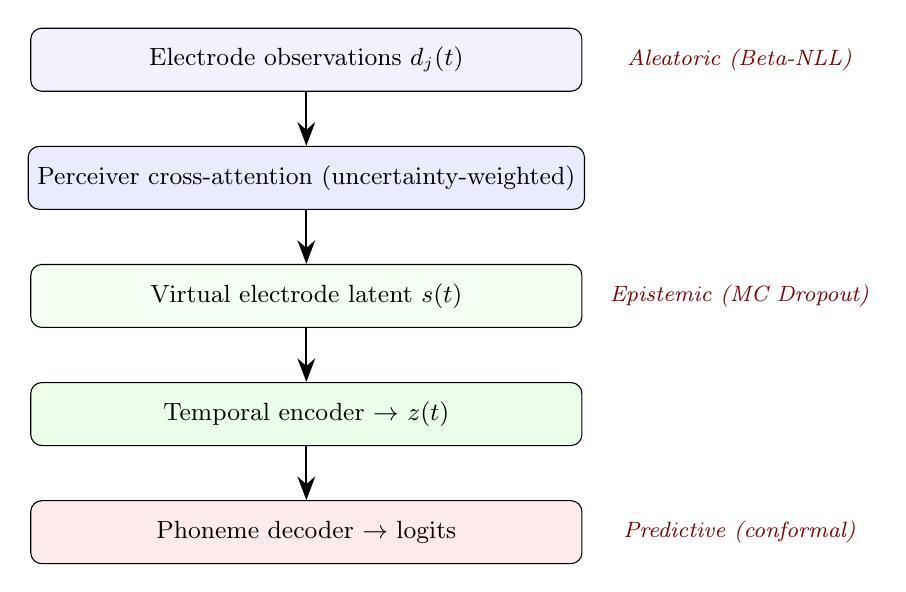
\begin{tikzpicture}[
  box/.style={draw, rounded corners, minimum width=7cm, minimum height=0.8cm, align=center, font=\small},
  uq/.style={font=\footnotesize\itshape, text=Maroon},
  arrow/.style={-{Stealth[length=3mm]}, thick}
]

\node[box, fill=blue!5] (elec) at (0, 0) {Electrode observations $d_j(t)$};
\node[uq] (uq1) at (5.5, 0) {Aleatoric (Beta-NLL)};

\node[box, fill=blue!8] (perceiver) at (0, -1.5) {Perceiver cross-attention (uncertainty-weighted)};

\node[box, fill=green!5] (latent) at (0, -3) {Virtual electrode latent $s(t)$};
\node[uq] (uq2) at (5.5, -3) {Epistemic (MC Dropout)};

\node[box, fill=green!8] (temporal) at (0, -4.5) {Temporal encoder $\to$ $z(t)$};

\node[box, fill=red!8] (phoneme) at (0, -6) {Phoneme decoder $\to$ logits};
\node[uq] (uq3) at (5.5, -6) {Predictive (conformal)};

\draw[arrow] (elec) -- (perceiver);
\draw[arrow] (perceiver) -- (latent);
\draw[arrow] (latent) -- (temporal);
\draw[arrow] (temporal) -- (phoneme);

\end{tikzpicture}
\end{center}

Each level captures a different source: \textbf{electrode level}---signal quality (impedance, contact, noise); \textbf{field level}---coverage gaps (no electrodes nearby); \textbf{prediction level}---phoneme ambiguity (articulatory similarity).


%% ====================================================================
%%  PART III: ARCHITECTURE
%% ====================================================================

\part{Architecture Design}

\section{Design Principles}

Every architectural choice traces back to the observation function:
\begin{equation}
d_j^{(i)}(t) = g(\bfp_j^{(i)} + \Delta^{(i)},\; \bfz(t);\; e^{(i)}) + \epsilon_j^{(i)}(t)
\end{equation}

\begin{table}[h]\centering\small
\begin{tabular}{@{}lll@{}}
\toprule
\textbf{Symbol} & \textbf{Meaning} & \textbf{Architectural component} \\
\midrule
$d_j^{(i)}(t)$ & Electrode observation & Input token \\
$\bfp_j^{(i)}$ & MNI position (approximate) & MNI positional encoding \\
$\Delta^{(i)}$ & Registration correction & Learnable 3D offset \\
$\bfz(t)$ & Shared articulatory state & Spatial encoder output \\
$e^{(i)}$ & Patient residual & Learnable embedding \\
$g(\cdot)$ & Shared somatotopic map & Observation decoder \\
$\epsilon$ & Noise & Regularization \\
\bottomrule
\end{tabular}
\end{table}

Four modules, each solving one subproblem:
\begin{enumerate}[leftmargin=2em]
\item \textbf{Spatial Encoder}---Invert $g$: observations at known positions $\to$ latent state $\hat{\bfz}(t)$
\item \textbf{Observation Decoder}---Implement $g$: latent state + position $\to$ predicted observation
\item \textbf{Temporal Encoder}---Model dynamics: $\hat{\bfz}(1{:}T) \to$ temporally-coded representations
\item \textbf{Phoneme Decoder}---Classify trajectory: temporal representations $\to$ phoneme sequence
\end{enumerate}


\section{Spatial Encoder (${\sim}$100K params)}

\subsection{Electrode tokens}

For electrode $j$ on patient $i$ at time $t$:
\begin{equation}
\text{token}_j = \underbrace{\text{Linear}(d_j \to d)}_{\text{activity}} + \underbrace{\text{Linear}(\bfp_j + \Delta^{(i)} \to d)}_{\text{MNI PE}} + \underbrace{\text{Linear}(\text{row}_j, \text{col}_j \to d)}_{\text{Grid PE}} + \underbrace{e^{(i)}}_{\text{patient}}
\end{equation}

\textbf{Per-patient parameters} ($3 + d = 67$ per patient):
\begin{itemize}[leftmargin=2em]
\item $\Delta^{(i)} \in \R^3$: learnable MNI offset (registration correction), initialized to $\mathbf{0}$.
\item $e^{(i)} \in \R^d$: learnable patient embedding, initialized $\sim \mathcal{N}(0, 0.02)$.
\end{itemize}

Dead electrodes are excluded from the token set (not masked, just absent). Variable $N_i$ is handled natively by attention.

\subsection{Perceiver cross-attention with distance bias}

$L = 16$ \textbf{virtual electrodes} with learnable MNI positions, initialized to cover the convex hull of source patient electrode positions:
\begin{equation}
\text{query}_i = \text{embed}_i + \text{MNI\_PE}(\text{v\_pos}_i)
\end{equation}

Cross-attention with spatial locality prior:
\begin{equation}
\boxed{A_{ij} = \frac{Q_i \cdot K_j}{\sqrt{d}} \;-\; \alpha \cdot \|\text{v\_pos}_i - (\bfp_j + \Delta^{(i)})\|^2}
\end{equation}
where $\alpha > 0$ is learnable (initialized 0.1), controlling spatial blur: large $\alpha =$ sharp attention (precise MNI trust), small $\alpha =$ fuzzy (robust to misalignment).

4-head attention, optional 1-layer self-attention (captures inter-zone interactions like lip-tongue co-articulation), then \textbf{MaxPool} across $L$ virtual outputs $\to s(t) \in \R^d$.

\subsection{Dimensions and parameter count}

\begin{table}[h]\centering\small
\begin{tabular}{@{}lrl@{}}
\toprule
\textbf{Component} & \textbf{Params} & \textbf{Notes} \\
\midrule
Activity embedding Linear($1 \to d$) & 128 & \\
MNI PE Linear($3 \to d$) & 256 & \\
Grid PE Linear($2 \to d$) & 192 & \\
Virtual electrode embeddings ($16 \times d$) & 1,024 & \\
Virtual MNI positions ($16 \times 3$) & 48 & \\
Cross-attention QKV + output ($4$ heads) & ${\sim}$16,384 & \\
Self-attention (1 layer) & ${\sim}$16,384 & \\
LayerNorm $\times 2$ & 256 & \\
FFN ($d \to 4d \to d$) $\times 2$ & ${\sim}$65,536 & \\
Distance scale $\alpha$ & 1 & \\
\midrule
\textbf{Total spatial encoder} & $\mathbf{{\sim}100}$\textbf{K} & \\
Per-patient $\Delta + e$ & 67/patient & \\
\bottomrule
\end{tabular}
\end{table}


\section{Observation Decoder (${\sim}$25K params)}\label{sec:obs-decoder}

The forward observation model---the ``renderer'' in the multi-view analogy:
\begin{equation}\label{eq:bilinear}
\boxed{\hat{d}_j(t) = \phi(\bfp_j + \Delta^{(i)},\; e^{(i)})^\top \;\psi(s(t))}
\end{equation}
\begin{itemize}[leftmargin=2em]
\item $\phi = \text{MLP}_{\text{spatial}}(\bfp, e) \in \R^k$: spatial tuning vector---encodes what articulatory features position $\bfp$ is sensitive to.
\item $\psi = \text{MLP}_{\text{latent}}(s) \in \R^k$: articulatory activation---encodes which tuning profiles are excited by the current state.
\item $k = 32$: bilinear interaction dimensionality.
\end{itemize}

\textbf{Interpretation}: $\phi$ is the somatotopic map at position $\bfp$; $\psi$ is the articulatory configuration. Their inner product gives predicted activity. This bilinear form is physically motivated by the separability of spatial tuning and articulatory dynamics (cf.\ MMGN, ICLR 2024).

\textbf{Reprojection loss} (self-supervised, no labels):
\begin{equation}\label{eq:reproj}
\mathcal{L}_{\text{reproj}} = \frac{1}{N_i} \sum_{j=1}^{N_i} \bigl\| d_j(t) - \hat{d}_j(t) \bigr\|^2
\end{equation}

This loss simultaneously trains: the spatial encoder to produce accurate $\hat{\bfz}(t)$; the observation decoder to learn the somatotopic map $g$; $\Delta^{(i)}$ to correct MNI registration error; and $e^{(i)}$ to capture patient-specific characteristics. \textbf{No phoneme labels are required.}

\textbf{With Beta-NLL} (uncertainty-aware, Section~\ref{sec:uncertainty}):
\begin{equation}
\mathcal{L}_{\text{reproj}}^{\text{UQ}} = \frac{1}{N_i} \sum_{j} \frac{1}{2}\Bigl(\log \hat{\sigma}_j^2 + \frac{(d_j - \hat{d}_j)^2}{\hat{\sigma}_j^2}\Bigr) \cdot (\hat{\sigma}_j^2)^{0.5}_{\text{sg}}
\end{equation}
where $\hat{\sigma}_j^2$ is the predicted per-electrode variance and ``sg'' denotes stop-gradient.

\textbf{Electrode masking}: During training, randomly drop 20--40\% of electrodes from encoder input but retain them in the reprojection loss. The model must spatially interpolate through the neural field---geometric masked reconstruction grounded in the observation model.


\section{Temporal Encoder (${\sim}$70K params)}

\subsection{Multi-scale tokenization (experimentally validated)}

\begin{equation}
\begin{aligned}
s(1{:}T) &\xrightarrow{\text{Conv1d}(d,d,k{=}3,s{=}3)} T_3 \approx 67 \text{ tokens at } {\sim}67\,\text{Hz} \quad \text{(fast transitions)}\\
s(1{:}T) &\xrightarrow{\text{Conv1d}(d,d,k{=}5,s{=}5)} T_5 \approx 40 \text{ tokens at } {\sim}40\,\text{Hz} \quad \text{(syllable dynamics)}\\
s(1{:}T) &\xrightarrow{\text{Conv1d}(d,d,k{=}10,s{=}10)} T_{10} \approx 20 \text{ tokens at } {\sim}20\,\text{Hz} \quad \text{(phoneme-level)}
\end{aligned}
\end{equation}

All ${\approx}127$ tokens concatenated with learnable per-scale embeddings + sinusoidal temporal PE.

\subsection{Temporal transformer}

2 layers, 4 heads, $d{=}64$, FFN dim 256. Standard pre-norm transformer. Each token attends across all scales and times---the 67\,Hz token at $t{=}100$\,ms can attend to the 20\,Hz token at $t{=}800$\,ms.

\subsection{Readout}

For $k$-NN evaluation: $z_{\text{global}} = \text{mean\_pool}(\text{all 127 tokens}) \in \R^d$. For per-position classification: $z_{\text{pos}} = \text{mean\_pool}(\text{tokens within each phoneme window}) \in \R^d$ per position (windows: 0--333ms, 333--666ms, 666--1000ms).


\section{Phoneme Decoder (${\sim}$5K params)}

\textbf{Dual head} (experimentally validated):
\begin{equation}
\text{logits}_p = \frac{1}{2}\bigl(\underbrace{\text{Linear}(z \to 9)}_{\text{CE head}} + \underbrace{\tau \cdot \text{normalize}(\text{Linear}(z \to 15)) \cdot A^\top}_{\text{articulatory head}}\bigr)
\end{equation}
where $A \in \R^{9 \times 15}$ is the fixed articulatory feature matrix and $\tau$ is a learnable temperature.

\textbf{Classification loss}:
$\mathcal{L}_{\text{class}} = \frac{1}{3}\sum_{p=1}^{3} \text{FocalCE}(\text{logits}_p, y_p;\; \gamma{=}2, \text{LS}{=}0.1)$
with mixup ($\alpha{=}0.2$).


\section{Complete Architecture}

\begin{center}
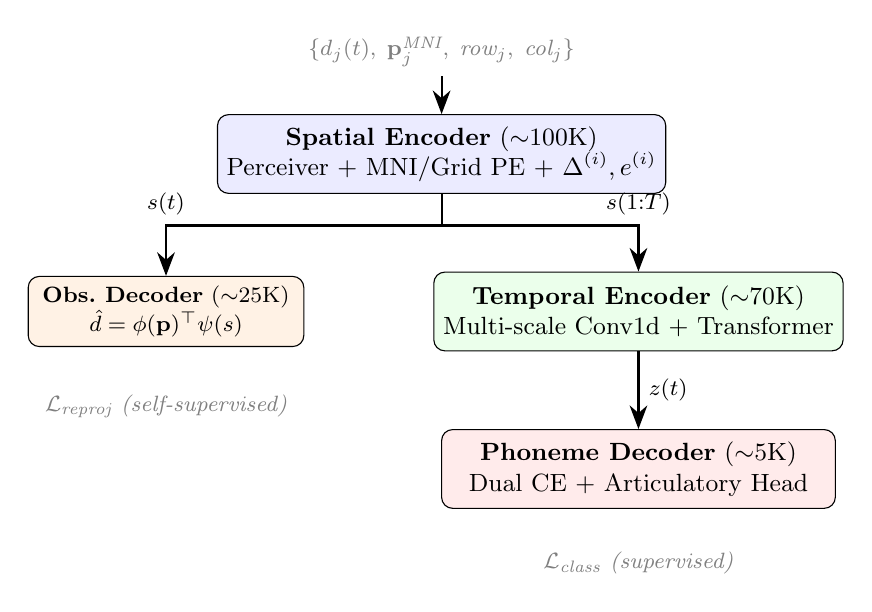
\begin{tikzpicture}[
  box/.style={draw, rounded corners, minimum width=5cm, minimum height=1cm, align=center, font=\small},
  smallbox/.style={draw, rounded corners, minimum width=3.5cm, minimum height=0.8cm, align=center, font=\footnotesize},
  arrow/.style={-{Stealth[length=3mm]}, thick},
  label/.style={font=\footnotesize\itshape, text=gray}
]

\node[box, fill=blue!8] (spatial) at (0, 0) {\textbf{Spatial Encoder} (${\sim}$100K)\\Perceiver + MNI/Grid PE + $\Delta^{(i)}, e^{(i)}$};

\node[smallbox, fill=orange!10] (obs) at (-3.5, -2) {\textbf{Obs.\ Decoder} (${\sim}$25K)\\$\hat{d} = \phi(\bfp)^\top\psi(s)$};

\node[box, fill=green!8] (temporal) at (2.5, -2) {\textbf{Temporal Encoder} (${\sim}$70K)\\Multi-scale Conv1d + Transformer};

\node[box, fill=red!8] (phoneme) at (2.5, -4) {\textbf{Phoneme Decoder} (${\sim}$5K)\\Dual CE + Articulatory Head};

\node[label] (input) at (0, 1.3) {$\{d_j(t),\; \bfp_j^{\text{MNI}},\; \text{row}_j,\; \text{col}_j\}$};

\draw[arrow] (input) -- (spatial);
\draw[arrow] (spatial.south) -- ++(0,-0.4) -| (obs.north) node[midway, above, font=\footnotesize] {$s(t)$};
\draw[arrow] (spatial.south) -- ++(0,-0.4) -| (temporal.north) node[midway, above, font=\footnotesize] {$s(1{:}T)$};
\draw[arrow] (temporal) -- (phoneme) node[midway, right, font=\footnotesize] {$z(t)$};

\node[label] at (-3.5, -3.2) {$\mathcal{L}_{\text{reproj}}$ (self-supervised)};
\node[label] at (2.5, -5.2) {$\mathcal{L}_{\text{class}}$ (supervised)};

\end{tikzpicture}
\end{center}

\begin{equation}
\boxed{\mathcal{L} = \mathcal{L}_{\text{class}} + \lambda \cdot \mathcal{L}_{\text{reproj}}}
\end{equation}

\begin{table}[h]\centering\small
\begin{tabular}{@{}lrl@{}}
\toprule
\textbf{Module} & \textbf{Params} & \textbf{Role} \\
\midrule
Spatial encoder & ${\sim}$100K & Invert observation function \\
Observation decoder & ${\sim}$25K & Forward model (reprojection) \\
Temporal encoder & ${\sim}$70K & Dynamics modeling \\
Phoneme decoder & ${\sim}$5K & Classification \\
\midrule
\textbf{Total shared} & $\mathbf{{\sim}200}$\textbf{K} & \\
Per-patient ($\times 10$) & 670 & Registration + identity \\
\textbf{Grand total} & $\mathbf{{\sim}201}$\textbf{K} & (cf.\ current pipeline: 122K) \\
\bottomrule
\end{tabular}
\end{table}


%% ====================================================================
%%  PART IV: TRAINING, EVALUATION, AND EXPERIMENTAL DESIGN
%% ====================================================================

\part{Training, Evaluation, and Experimental Design}

\section{Training Pipeline}

\subsection{Phase 1: Source patient training (supervised + reprojection)}

9 source patients, ${\sim}1315$ labeled trials. Each batch:
\begin{enumerate}[leftmargin=2em]
\item \textbf{Spatial encoding}: construct electrode tokens with dual PE + patient params, mask 20--40\% electrodes, Perceiver cross-attention $\to s(t)$ per frame.
\item \textbf{Reprojection}: observation decoder predicts all electrodes (including masked); $\mathcal{L}_{\text{reproj}}$ (or $\mathcal{L}_{\text{reproj}}^{\text{UQ}}$ with Beta-NLL).
\item \textbf{Temporal encoding}: $s(1{:}T) \to$ multi-scale Conv1d $\to$ temporal transformer $\to z(t)$.
\item \textbf{Classification}: dual head $\to \mathcal{L}_{\text{class}}$ with focal CE, label smoothing, mixup.
\item \textbf{Total}: $\mathcal{L} = \mathcal{L}_{\text{class}} + \lambda \mathcal{L}_{\text{reproj}}$ with $\lambda$: $0.5 \to 0.1$ annealed.
\end{enumerate}

\textbf{Optimizer}: AdamW with differential LR:
\begin{itemize}[leftmargin=2em]
\item Shared parameters: $\text{lr} = 10^{-3}$
\item Virtual electrode positions: $\text{lr} = 3 \times 10^{-4}$ (slow---positions should stabilize)
\item Per-patient $\Delta$: $\text{lr} = 3 \times 10^{-4}$ (slow---geometric correction)
\item Per-patient $e$: $\text{lr} = 10^{-3}$ (can adapt faster)
\end{itemize}

Linear warmup (20 epochs) $\to$ cosine decay. Weight decay $10^{-4}$. Gradient clipping 5.0. Batch size 16. Early stopping on held-out 20\% source validation, patience 7.

\textbf{Optional extension}: Alternate labeled batches (both losses) with unlabeled batches from continuous recordings or Lexical patients (reprojection only---no labels needed).

\subsection{Phase 2: Target adaptation (LP-FT)}

Per CV fold on target patient (5-fold grouped-by-token):
\begin{enumerate}[leftmargin=2em]
\item \textbf{Linear probe} (freeze encoder): Initialize $\Delta^{(\text{target})} = 0$, $e^{(\text{target})} = \text{mean}(e^{(\text{source})})$. Train phoneme decoder + $\Delta$ + $e$ only. 150 epochs.
\item \textbf{Fine-tune} (unfreeze): Unfreeze spatial + temporal encoder at $0.1\times$ LR. Continue all params. 100 epochs, patience 7.
\end{enumerate}

\subsection{Phase 3 (optional): Reprojection pre-training}

Pre-train spatial encoder + observation decoder on all available data (continuous recordings + Lexical patients) using $\mathcal{L}_{\text{reproj}}$ only. No phoneme labels needed. Then initialize Phase~1 from pre-trained weights. This is the SSL component---grounded in the reprojection objective rather than arbitrary masked prediction.


\section{Evaluation Protocol}

\textbf{Primary metric}: PER via edit distance, grouped-by-token 5-fold CV.

\textbf{Full evaluation recipe} (all experimentally validated):

\begin{table}[h]\centering\small
\begin{tabular}{@{}lll@{}}
\toprule
\textbf{Component} & \textbf{Setting} & \textbf{Source} \\
\midrule
Weighted $k$-NN & $k{=}10$, cosine similarity & Autoresearch exp9 \\
TTA & 16 augmented copies & Autoresearch exp16 \\
Dual head & CE + articulatory, averaged & Autoresearch exp14--15 \\
Best-of per fold & $\min(\text{linear}, \text{kNN})$ per fold & Autoresearch exp9 \\
Source $k$-NN & Source embeddings at $0.5\times$ weight & LOPO exp13 \\
\midrule
Conformal prediction & Coverage-guaranteed prediction sets & Section~\ref{sec:uncertainty} \\
MC Dropout & 10--20 passes for epistemic UQ & Section~\ref{sec:uncertainty} \\
\bottomrule
\end{tabular}
\end{table}


\section{Ablation Experiments}

\begin{table}[h]\centering\small
\begin{tabular}{@{}clp{7.5cm}@{}}
\toprule
\textbf{ID} & \textbf{Ablation} & \textbf{Question} \\
\midrule
A1 & MNI PE present/absent & \textbf{Central question}: do MNI coordinates help? \\
 & \quad a. Current Conv2d + BiGRU baseline & $\to$ PER 0.762 \\
 & \quad b. Perceiver + Grid PE only (no MNI) & $\to$ architecture benefit \\
 & \quad c. Perceiver + MNI PE only (no Grid) & $\to$ MNI benefit \\
 & \quad d. Perceiver + MNI + Grid PE & $\to$ combined benefit \\
 & \quad e. (d) + reprojection loss & $\to$ reprojection benefit \\
\midrule
A2 & Population-level (all patients) & Is the 0.76 wall S14-specific or universal? \\
A3 & Per-patient params ($\Delta$/$e$/both/neither) & Which per-patient parameters matter? \\
A4 & Virtual electrode count ($L \in \{4, 8, 16, 32\}$) & How many virtual electrodes needed? \\
A5 & Reprojection weight ($\lambda \in \{0, 0.01, 0.1, 0.5\}$) & Does reprojection help or hurt classification? \\
A6 & Cross-task pooling (Duraivel data) & Does more data help? (architecture-independent) \\
A7 & Uncertainty stack (Beta-NLL vs.\ MSE reproj) & Does learned variance improve convergence? \\
\bottomrule
\end{tabular}
\end{table}


\section{Available Data and Experimental Paths}

\subsection{Currently used}

\begin{table}[h]\centering\small
\begin{tabular}{@{}lll@{}}
\toprule
\textbf{Data source} & \textbf{Volume} & \textbf{Usage} \\
\midrule
PS task trial-level HGA & 9 patients, ${\sim}1315$ trials & Supervised LOPO training \\
S14 trial-level HGA & 153 trials & Target patient evaluation \\
Grid topology (from TSV) & Per-patient & SpatialConv input structure \\
\bottomrule
\end{tabular}
\end{table}

\subsection{Available but unused}

\begin{table}[h]\centering\small
\begin{tabular}{@{}lllc@{}}
\toprule
\textbf{Data source} & \textbf{Volume} & \textbf{Potential usage} & \textbf{Risk} \\
\midrule
Cross-task pooling (Duraivel) & 3 patients, 156--208 trials & Doubles labeled data & Low \\
MNI coordinates & All patients & Spatial alignment & Medium \\
Continuous recordings & ${\sim}168$\,min & Reprojection SSL & Medium \\
Lexical task patients & 13 patients & Additional sources & Medium \\
Audio recordings & 4 variants/patient & Auxiliary supervision & Medium \\
\bottomrule
\end{tabular}
\end{table}

\textbf{Highest priority}: Cross-task pooling (same tokens, same phonemes, overlapping patients, compatible preprocessing). \textbf{Hard dependency}: MNI coordinate sourcing from BioImage Suite / Brainlab / ECoG\_Recon on Box. \textbf{Lower priority}: Continuous recording extraction + VAD curation for Phase~3 reprojection SSL. The continuous data caveat: ${\sim}168$ minutes are dominated by silence, OR ambient noise, and anesthesia fluctuations; aggressive curation required.


\section{MNI Coordinate Sourcing}

The architecture requires MNI-152 coordinates per electrode. Current pipeline uses ACPC-normalized grid positions (0--1 range in TSVs) for grid topology only.

\textbf{Where they likely are}: BioImage Suite outputs (DBS patients), Brainlab outputs (tumor patients), ECoG\_Recon data on Box, BIDS coordsystem JSON files.

\textbf{Fallbacks}: (1) Use ACPC grid positions scaled to approximate mm---loses cross-patient alignment but retains within-patient structure. (2) Estimate MNI from grid positions + array metadata (center in MNI from surgical reports + grid geometry).


\section{Risk Assessment}

\begin{table}[h]\centering\small
\begin{tabular}{@{}p{0.35\textwidth}cp{0.42\textwidth}@{}}
\toprule
\textbf{Risk} & \textbf{Severity} & \textbf{Mitigation} \\
\midrule
MNI coordinates unavailable & High & Fallback to scaled ACPC + Grid PE only \\
MNI alignment too imprecise & High & Ablation A1; learnable $\alpha$ adapts spatial blur \\
Reprojection hurts classification & Medium & $\lambda$ ablation A5; can set $\lambda{=}0$ \\
Perceiver overfits (200K on 1300 trials) & Medium & Reprojection regularizes; masking; early stopping \\
Virtual electrodes collapse & Low & Initialize across convex hull; monitor \\
Per-patient $\Delta$ overfits & Low & L2 penalty; low learning rate \\
\bottomrule
\end{tabular}
\end{table}


\section{Success Criteria}

\begin{table}[h]\centering\small
\begin{tabular}{@{}lp{9cm}@{}}
\toprule
\textbf{Level} & \textbf{Criterion} \\
\midrule
Minimum & A1d (Perceiver + MNI + Grid) outperforms A1b (Grid only) by ${\geq}2\pp$ on S14 \\
Target & PER ${<}$ 0.740 on S14 (exceeds per-patient supervised 0.737) \\
Strong & Population-level improvement across all patients \\
Interpretability & Virtual electrodes cluster over vSMC; $\Delta^{(i)}$ larger for tumor patients; $\phi(\bfp)$ recovers somatotopy \\
\bottomrule
\end{tabular}
\end{table}


\section{Summary}

This document formalizes cross-patient speech decoding as \textbf{multi-view neural field reconstruction}: multiple patients observe the same cortical dynamics from different electrode positions, analogous to multiple cameras observing the same 3D scene.

The theoretical foundation rests on three claims of increasing specificity:
\begin{enumerate}[leftmargin=2em]
\item \textbf{Externally established}: Articulatory somatotopy exists in vSMC (Metzger, Bouchard); motor cortex manifold dynamics are preserved across individuals (Safaie, Gallego); per-patient input + shared backbone is optimal for transfer (Singh, Willett); MNI coordinates enable cross-patient ECoG decoding (Chen/SwinTW).
\item \textbf{Internally observed}: LOPO transfer works (PER 0.762); articulatory bottleneck and multi-scale temporal encoding improve performance; 55 experiments converge to PER 0.750--0.780.
\item \textbf{Working hypothesis}: The shared observation function $g(\bfp, \bfz)$ factorizes the somatotopic map from articulatory dynamics, and MNI coordinates can align this function across patients.
\end{enumerate}

The Neural Field Perceiver implements this framework: Perceiver cross-attention with MNI distance bias inverts the observation function (${\sim}100$K), a bilinear observation decoder implements it forward for reprojection (${\sim}25$K), a multi-scale temporal transformer models articulatory dynamics (${\sim}70$K), and per-position dual heads decode phonemes (${\sim}5$K). Three-level uncertainty estimation (Beta-NLL, MC Dropout, conformal prediction) provides per-electrode, per-position, and per-prediction confidence. Every architectural component has a validated analog in the 2024--2026 3D vision literature.

Total budget: ${\sim}200$K shared parameters + 67 per patient. The architecture directly maps every component to the observation equation $d_j^{(i)}(t) = g(\bfp_j^{(i)} + \Delta^{(i)}, \bfz(t); e^{(i)}) + \epsilon_j^{(i)}(t)$.

\end{document}
